\section{Prediction and Parsimony}

We took 20 UCI data sets and created 1000 permutations of each data set.
We then took the first $x$\% of each permuted data set ($x$ in
${10,20,30,\ldots,90}$) as training data and used the remaining part as
test data. We used exact structure learning to learn the best
scoring model using BDeu ($\alpha=1$), BIC, fNML and qNML,
recording the number of parameters in the learnt
models and the average predictive log-probability of each test
vector. These numbers are collected for 1000 different data
permutations, the average and variance of which appear on the following
pages, one page per data set.

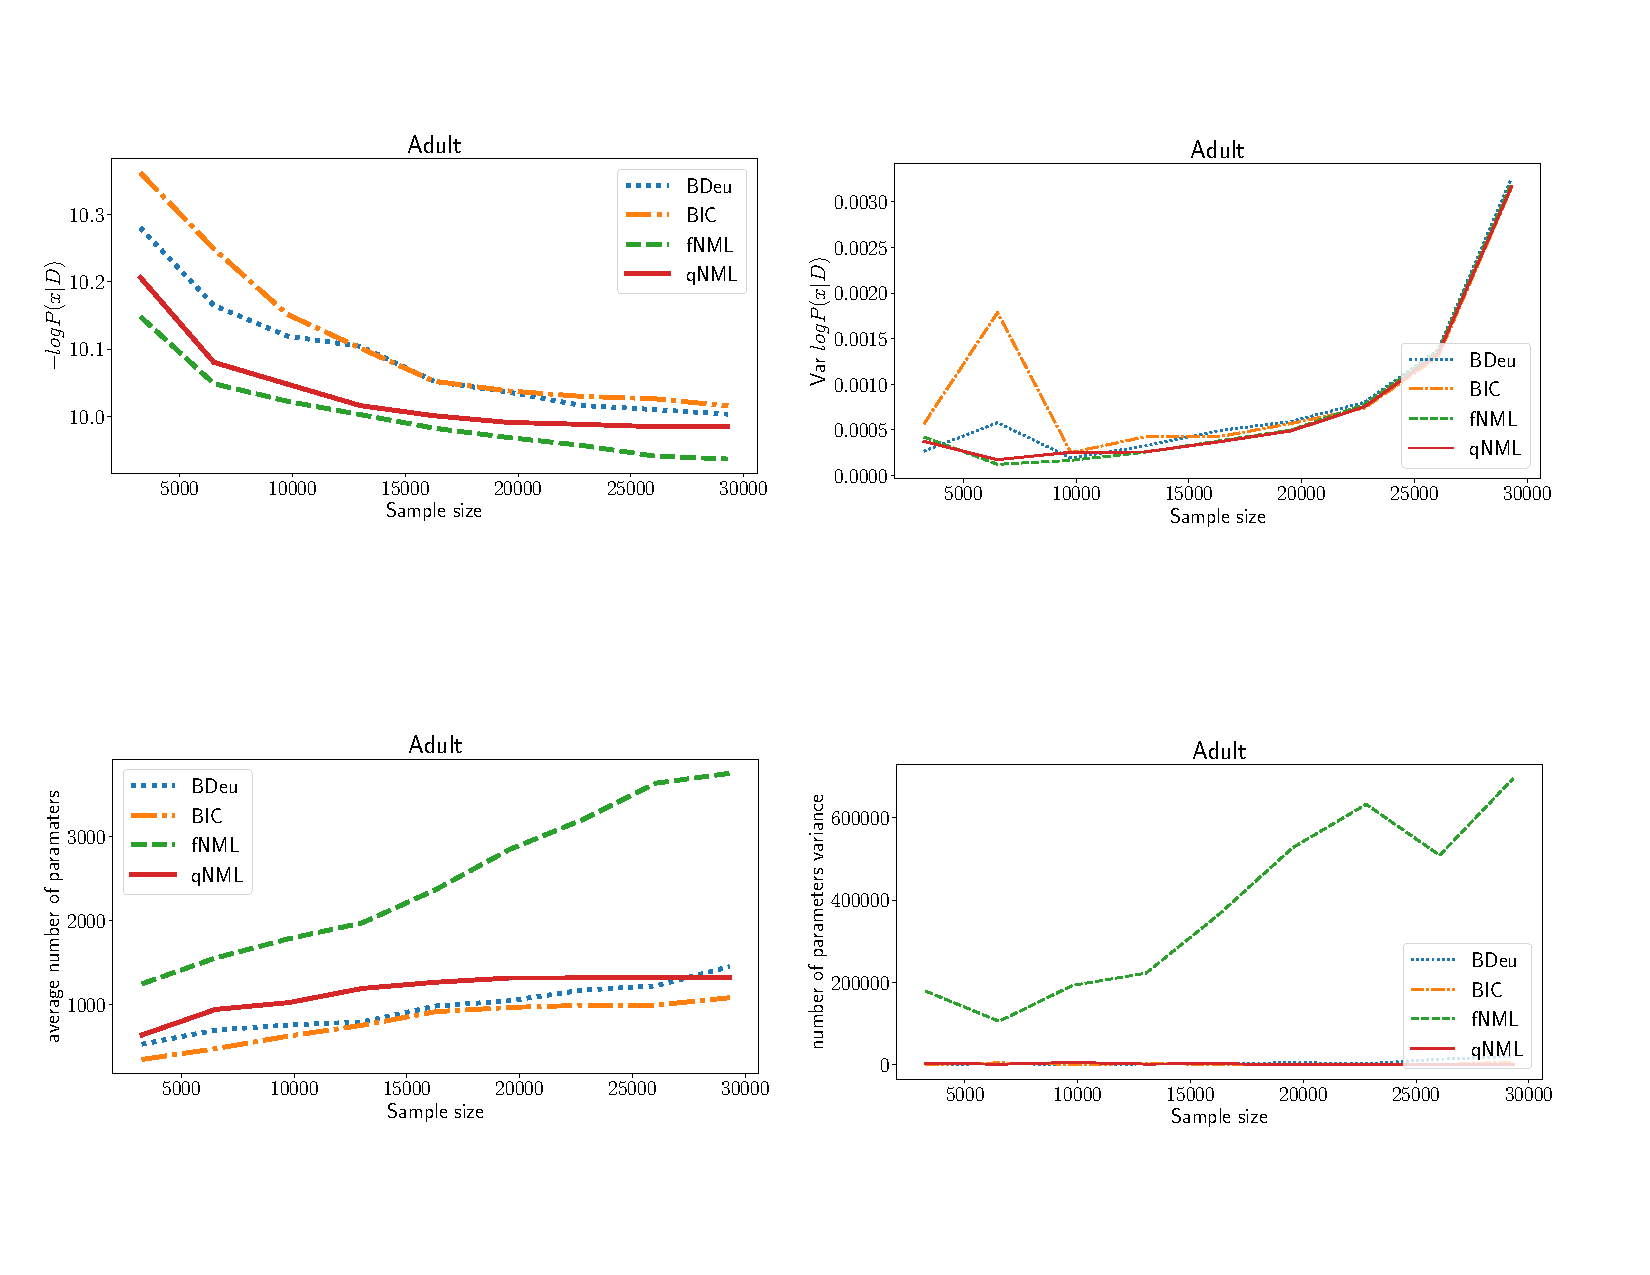
\includepdf[pages={1-20}]{all_qNML_images4.pdf}
